\documentclass[12pt, a4paper]{article}

\usepackage[utf8]{inputenc}
\usepackage[T1]{fontenc}
\usepackage[russian]{babel}
\usepackage[oglav,spisok,boldsect, figwhole]{./style/fn2kursstyle1}
\graphicspath{{./style/}{./figures/}}
%\usepackage{float}%"Плавающие" картинки
\usepackage{multirow}
\usepackage{subcaption}
\usepackage{float}%"Плавающие" картинки
%Римские цифры
\newcommand{\RomanNumeralCaps}[1]
{\MakeUppercase{\romannumeral #1}}

\usepackage{enumitem} 
\usepackage{amsmath}
\usepackage{comment}
\usepackage{makecell}

%Параметры титульника
\title{Методы решения нелинейных уравнений}
\group{ФН2-52Б}
\author{Г.А.~Швецов}
\supervisor{А.О.~Гусев}
\date{2022}
\begin{document}
	\newcommand{\pl}{\partial}
	\maketitle
	
	\tableofcontents
	
	\newpage
	
	\section{Контрольные вопросы}
	% TODO %%%%%%%%%%%%%%%%%%%%%%%%%%%%%%%%%%%%%%%%%%%%%%%%%%%%
	\begin{enumerate}
		\item \textit{Можно ли использовать методы бисекции и Ньютона для нахождения кратных корней уравнения $f (x) = 0$ (т.е. тех, в которых одна или несколько первых производных функций $f (x)$ равны нулю)? Обоснуйте ответ.}
		\smallskip
		
		Метод бисекции применим в случае нечетной кратности корня, т.к. только в этом случае выполнено условие $f(a) \cdot f(b)<0$.
				
			Метод Ньютона применим для поиска корней любой кратности. В случае кратности более 1 скорость сходимости линейна.
		
		% Доказательство при произвольной кратности p есть в Самарском, численные методы на стр. 202 (хотя там про другое, но может быть полезным)
		\textbf{Доказательство:}
		
		Итерационная формула метода Ньютона:
	\begin{equation}
		\label{Newton}
		x^{(k+1)} = x^{(k)} - \dfrac{f(x^{(k)})}{f'(x^{(k)})}.
	\end{equation}
	
	Пусть корень $x^*$ уравнения $f(x)=0$ имеет кратность 2. Получаем, что $f(x_*) = f'(x^*) = 0$. Разложим функцию $f(x)$ и ее производную $f'(x)$ в ряд Тейлора в точках $x^{(k)}$ и $x^*$ соответственно и подставим $x = x^*$ и $x = x^{(k)}$. Тогда с учетом предыдущих равенств получаем, что
	\begin{eqnarray}
		\label{eq1}
		& f(x^*) = f(x^{(k)}) + f'(x^{(k)}) (x^*-x^{(k)}) + \frac12 f''(\xi_k) (x^*-x^{(k)})^2,\; \xi \in [x^*, x^{(k)}]; \\
		\label{eq2}
		& f'(x^{(k)}) = f'(x^*) + f''(\eta_k) (x^{(k)}-x^*) = f''(\eta_k) (x^{(k)}-x^*), \; \eta \in [x^{(k)}, x^*].
	\end{eqnarray}
	
	Выражая из выражения \eqref{eq1} $f(x^{(k)})$ и подставляя результаты в формулу \eqref{Newton}, получаем:
	\begin{multline*}
		x^{(k+1)} = x^{(k)} - \frac{-\left(f'(x^{(k)}) (x_*-x^{(k)}) + \frac12 f''(\xi_k) (x^*-x^{(k)})^2\right)}{f'(x^{(k)})} = x^{(k)} + (x^* - x^{(k)}) +\\
		+\frac{\frac12 f''(\xi_k) (x^*-x^{(k)})^2}{f'(x^{(k)})} = x^* + \frac{\frac12 f''(\xi_k) (x^*-x^{(k)})^2}{f''(\eta_k) (x^{(k)}-x^*)} = x^* + \frac12 \frac{f''(\xi_k)}{f''(\eta_k)} (x^* - x^{(k)}) \Rightarrow \\
		\Rightarrow |x^{(k+1)} - x^*| = \frac12 \left|\frac{f''(\xi_k)}{f''(\eta_k)}\right| |x^* - x^{(k)}| \Rightarrow |x^{(k+1)} - x^*| \le C | x^{(k)} - x^*|.
	\end{multline*}
	Таким образом, в данном случае метод Ньютона имеет линейную скорость сходимости.
	
	Чтобы улучшить скорость сходимости в случае кратного корня, можно использовать следующую модификацию метода Ньютона:
	\[
	x^{(k+1)} = x^{(k)} - p \frac{f(x^{(k)})}{f'(x^{(k)})}, \text{ где $p$ --- кратность корня}.
	\]
	% Еще можно применить метод Эйткена (Самарский, численные методы, стр. 198)
		
		\item \textit{При каких условиях можно применять метод Ньютона для
			поиска корней уравнения $f(x)=0,\, x \in [a,b]$? При каких ограничениях
			на функцию $f (x)$ метод Ньютона обладает квадратичной
			скоростью сходимости? В каких случаях можно применять метод Ньютона для решения систем нелинейных уравнений?}.
		\smallskip
		
		Функция $f(x)$ должна быть непрерывна-дифференцируема, т.е. $f(x)\in C^1$.
		
		Метод Ньютона обладает квадратичной скоростью сходимостью при следующих ограничениях ($f(x) = 0 \Leftrightarrow F(x) = x$):
		\[
		|f'(x)|\ge m > 0,\qquad |f''(x)|\le M,
		\]
		\[
		 |F'(x)| = \left|1- \frac{(f'(x))^2-f(x)f''(x)}{(f'(x))^2}\right|=\frac{|f(x)\cdot f''(x)|}{(f'(x))^2}<1,
		\]
		где $m$, $M$ --- константы, то при попадании очередного приближения $x^{(k)}$ в эту окрестность итерационный процесс по методу Ньютона будет сходиться с квадратичной скоростью
		\[
		|x^{(k+1)}-x^*|<C|x^{(k)}-x^*|^2, \qquad  k = s,\,s+1,\,s+2,\dots
		\]
		\textbf{Теорема (о достаточных условиях сходимости метода Ньютона)}.
		Пусть выполняются следующие условия:
		\begin{enumerate}
			\item Функция $f(x)$ определена и дважды дифференцируема на отрезке $[a,\,b]$;
			\item Отрезку $[a,\,b]$ принадлежит только один простой корень $x^*$, так что \\$f(a)\cdot f(b)<0$;
			\item Производные $f'(x),\,f''(x)$ на $[a,\,b]$ сохраняют знак, и $f'(x)\ne0$;
			\item Начальное приближение $x^{(0)}$ удовлетворяет неравенству $f(x^{(0)})\cdot f''(x^{(0)})\mbox{>0.}$
		\end{enumerate}
	Тогда с помощью метода Ньютона можно вычислить корень уравнения $f(x)\mbox{=0}$ с любой точностью.
	\smallskip
		\item \textit{Каким образом можно найти начальное приближение?}
		\smallskip
		
		Если известен отрезок $[a,b]$ локализации корня, то для получения начального приближения $x^{(0)}$ можно использовать \textit{метод хорд}
		\[
		x^{(0)} = \frac{f(a)\cdot b -f(b) \cdot a}{f(a) - f(b)},
		\]
		т.е. $x^{(0)}$ --- абсцисса точки пересечения с осью $Ox$ отрезка, соединяющего точки $(a,f(a))$ и $(b,f(b))$.
		
		Также в качестве начального приближения $x^{(0)}$ можно взять (\textit{метод бисекции})
		\[
		x^{(0)}=\frac{a+b}{2}.
				\]
		
		\item \textit{Можно ли использовать метод Ньютона для решения СЛАУ?}
		\smallskip
		
		СЛАУ имеет вид $Ax=b$. Обозначим $F(x) = Ax-b$, тогда $F'(x) = F' = A$.
		Тогда согласно итерационной формуле метода Ньютона
		\[
		X^{(k+1)} = X^{(k)}-(F'(X^{(k)})^{-1}F(X^{(k)}))=X^{(k)}-A^{-1}(AX^{(k)}-b)=A^{-1}b.
		\]
		Таким образом, метод Ньютона можно использовать для решения СЛАУ в том случае, если квадратная матрица $A$ имеет обратную $A^{-1}$.
		
		Метод сходится максимум за две итерации
		\[
		0 = \|X^{(2)} - X^{(1)}\|<\varepsilon.
		\]
		
		
		\item \textit{Предложите альтернативный критерий окончания итераций в методе бисекции, в котором учитывалась бы возможность попадания очередного приближения в очень малую окрестность корня уравнения.}
		\smallskip
		
		Можно сравнивать значения функции на концах и в середине отрезка с нулем.
		
		\item \textit{Предложите различные варианты модификаций метода Ньютона. Укажите их достоинства и недостатки.}
		\smallskip
		
		\begin{enumerate}
			\item \textbf{Упрощенный метод Ньютона (метод одной касательной)}. Вычисляем  производную функции или, в случае системы, матрицу Якоби только для первого приближения, т.е. итерационная формула метода Ньютона выглядит так
				\[
				x^{(k+1)} = x^{(k)}-\frac{f(x^{(k)})}{f'(x^{(0)})}, \qquad				
			X^{(k+1)} = X^{(k)}-(F'(X^{(0)}))^{-1}F(X^{(k)}).
			\]
			Данный метод по сравнению с классическим (квадратичная скорость) будет медленнее сходиться (линейная скорость), но все же он снижает вычислительные затраты (достаточно посчитать производную в точке $x^{(0)}$).
			\item \textbf{Метод секущих}. Замена производной в формуле Ньютона
			\[
			f'(x^{(k)}) \approx\frac{f(x^{(k-1)})-f(x^{(k)})}{x^{(k-1)} - x^{(k)}}
			\]  
			приводит к расчетной формуле
			\[
			x^{(k+1)} = x^{(k)}-f(x^{(k)})\frac{x^{(k-1)} - x^{(k)}}{f(x^{(k-1)})-f(x^{(k)})}.
			\]
			Метод является двухшаговым. Функция не обязана быть дифференцируемой, поэтому данный метод можно применять на широкий класс функций.
			\item \textbf{Метод Ньютона --- Бройдена}. Этот метод позволяет увеличить скорость сходимости последовательных приближений благодаря формуле
			\[
			x^{(k+1)} = x^{(k)}-c_k\frac{f(x^{(k)})}{f'(x^{(0)})},
			\]
			где $c_k$ --- число, которое выбирается на каждой итерации так, чтобы уменьшить значение $|f(x^{(k+1)})|$ по сравнению с $|f(x^{(k)})|$. Как правило, при плохой сходимости или ее отсутствии полагают $0<c_k<1$, а при хорошей сходимости для $c_k=1$ полагают $c_k>1$ (это ускоряет сходимость).
			\item \textbf{Метод Стеффенсена}. Итерационная формула метода Стеффенсена имеет вид
				\[
			x^{(k+1)} = x^{(k)}-\frac{f(x^{(k)})}{f(x^{(k)}+f(x^{(k)}))-f(x^{(k)})}.
			\]
			Метод Стеффенсена является одношаговым, не требует вычисления производной $f'(x)$ и в то же время, как и метод Ньютона, сходится с квадратичной скоростью. Метод Стффенсена уступает методу секущих, поскольку требует большей вычислительной работы.
			\item \textbf{Метод "замораживание через один"}. Итерационная формула одношагового метода имеет вид
			\begin{equation}
				x^{(k+1)} = x^{(k)}-\frac{f(x^{(k)})}{f'(x^{(k)})}-\frac{f\left(x^{(k)}-f(x^{(k)})(f'(x^{(k)}))^{-1}\right)}{f'(x^{(k)})}
				\label{e}
			\end{equation}
			
			
			Скорость сходимости данного метода является кубической.
			
			\textbf{Доказательство:}
			
			Формулу (\ref{e}) можно записать следующей системой
			\begin{equation}
			\begin{cases}
			y^{(k)} = x^{(k)}-\frac{f(x^{(k)})}{f'(x^{(k)})},\\
			x^{(k+1)}=y^{(k)}-\frac{f(y^{(k)})}{f'(x^{(k)})}.
			\end{cases}
			\label{system}
			\end{equation}
			Пусть $x*$ --- корень уравнения $f(x)=0$. Разложим функцию в ряд до третьего слагаемого (включительно)
			\begin{multline}
f(x^*) = f(x^{(k)}) + f'(x^{(k)}) (x^*-x^{(k)}) + \frac12 f''(x^{(k)}) (x_*-x^{(k)})^2+\\+\frac16 f'''(\xi_k)(x^*-x^{(k)})^3,\; \xi \in [x^*, x^{(k)}].
			\end{multline}
		Тогда 
		\[
		-\frac{f(x^{(k)})}{f'(x^{(k)})} = x^*-x^{(k)} + \frac12 \frac{f''(x^{(k)})}{f'(x^{(k)})} (x^*-x^{(k)})^2+\frac16 \frac{f'''(\xi_k)}{f'(x^{(k)})}(x^*-x^{(k)})^3,\; \xi \in [x^*, x^{(k)}].
		\]
		\newpage
		Подставляя это выражение в (\ref{system}), получаем
		\[
		y^{(k)} = x^*+\frac12 \frac{f''(x^{(k)})}{f'(x^{(k)})}(x^*-x^{(k)})^2+\frac16 \frac{f'''(\xi_k)}{f'(x^{(k)})}(x^*-x^{(k)})^3.
		\]
		Тогда
		\[
		|y^{(k)}-x^*| \le C|x^{(k)}-x^*|^2
		\]
		TODO
			\end{enumerate}
			
		
		
			\item \textit{Предложите алгоритм для исключения зацикливания метода Ньютона и выхода за пределы области поиска решения?}
		\smallskip
		
		Во избежание выхода очередного приближения за пределы отрезка можно использовать комбинацию алгоритмов Ньютона и метода хорд (в пределах --- метод Ньютона, за пределами --- метод хорд).
		
		Во избежании зацикливания через определенное количество итераций используем другой метод, например, метод бисекции.
		
		
		
		
	\end{enumerate}
	\newpage
	\section{Результаты}
	
	
	Функция: $x^2 - 4 \sin x + \ln(x+5)$
	
	Отрезок поиска: $-1 \le x \le 1$ 
	
	Точность: $\varepsilon = 0.001$
	
	Точное решение (вычисленное в Wolfram Mathematica): $0.516127723925248$
	
	Начальное приближение для метода Ньютона: $x^0 = -0.7$
	
	Оценка количества итераций для метода бисекции:
	\[\frac{b-a}{2^n} \le 2 \varepsilon, \quad 2^n \ge \frac{b-a}{2 \varepsilon}, \quad n \ge \log_2\frac{b-a}{2\varepsilon}.\]
	
	Оценка количества итераций для метода Ньютона:
		% Самарский, Гулин, Численные методы, 1989г., стр. 209, формула (10)
	\[
	|x^k - x_*| \le \frac{q^k}{1-q} \left|\frac{f(x^0)}{f'(x^0)}\right|, \text{ где } q = \max\limits_{x\in[a, b]} \left|\frac{f f''}{f'^2}\right|.
 		\]
	
	\begin{table}[H]
		\caption{Сравнение результатов методов}
	\centering
		\footnotesize
		\begin{tabular}{|p{1.9cm}|c|c|c|c|} \hline
		&\textbf{Метод хорд}	& \textbf{Метод бисекции} & \textbf{\makecell{Метод Ньютона,\\аналитич. произв.}} & \textbf{\makecell{Метод Ньютона,\\численная произв.}} \\ \hline
			
			\makecell{Результат} &0.516129712688983& 0.516601562500000 & 0.516127702953010 & 0.516127830340478 \\ \hline
			\makecell{Достигнутая\\точность} &0.000001988763735& 0.000473838574752 & 0.000000020972238 & 0.000000106415230 \\ \hline
			\makecell{Невязка} &0.000004505347242& 0.001072993704317 & 0.000000047510609 & 0.000000241073557 \\ \hline
			%Оценка трудоемкости  & 1 & 2 & 3 \\ \hline
			\makecell{Кол-во \\ итераций} &7& 10 & 4 & 4 \\ \hline
			\makecell{Оценка \\кол-ва\\итераций} &---& 10 &\multicolumn{2}{c|}{---} \\ \hline
			\makecell{Порядок \\ сходимости}& 1.641769886747711&1.311565782225854&1.993086440377016&1.582081537253162\\
			\hline
		\end{tabular}
\end{table}
	
	\begin{table}[H]
		\centering
		\caption{Квадратичная сходимость метода Ньютона}
\begin{tabular}{|c|c|c|}
	\hline
	\textbf{Итерации}&\textbf{\makecell{Метод Ньютона,\\аналитич. произв.}}&\textbf{\makecell{Метод Ньютона,\\численная произв.}}\\
	\hline
	1&0.370662064055730&0.370582289101866\\
	\hline
	2&\underline{0.5}02555503936164&\underline{0.5}02623170227612\\
	\hline
	3&\underline{0.515}972422772407&\underline{0.515}985168673437\\
	\hline
	4&\underline{0.5161277}02953010&\underline{0.516127}830340478\\
	\hline
\end{tabular}
	\end{table}
Подчеркиванием отмечены верные значащие цифры. Видно, что их количество от шага к шагу растет (приблизительно удваиваясь с каждым шагом), иллюстрируя квадратичную скорость сходимости.

При корне кратности 2 (на примере функции $f(x) = (x-1)^2$) порядок сходимости $p = 1.000000000000103$.

При корне кратности 2 (на примере функции $f(x) = (x-1)^2(x-3)^2$) порядок сходимости $p = 1.001024090561162$.

При корне кратности 2 (на примере функции $f(x) = (x-1)^2(x-3)^2$) порядок сходимости модифицированным методом $p = 1.997361522322007$.
\\\\
\begin{figure}[H]
	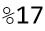
\includegraphics[width=\textwidth]{pool}
	\caption{Бассейн Ньютона ($300\times 300$ точек)}
\end{figure}





	
	
	\centering	
	\newpage
		Тест 4
	\[
	\begin{cases}
		x_1^2-x_2^2-15=0\\
		x_1x_2+4=0
	\end{cases}
	\]
	
	
	\begin{figure}[H]
		\centering
		\begin{subfigure}{0.45\textwidth}
			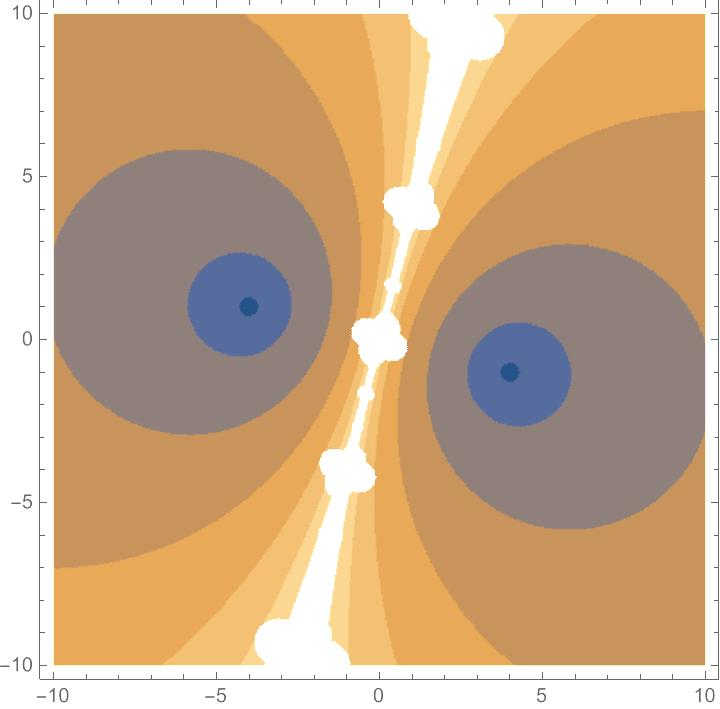
\includegraphics[width=\textwidth]{2D4}
			\caption{Область сходимости метода Ньютона "2D" (аналитическая производная)}
		\end{subfigure}
		\hfill
		\begin{subfigure}{0.45\textwidth}
			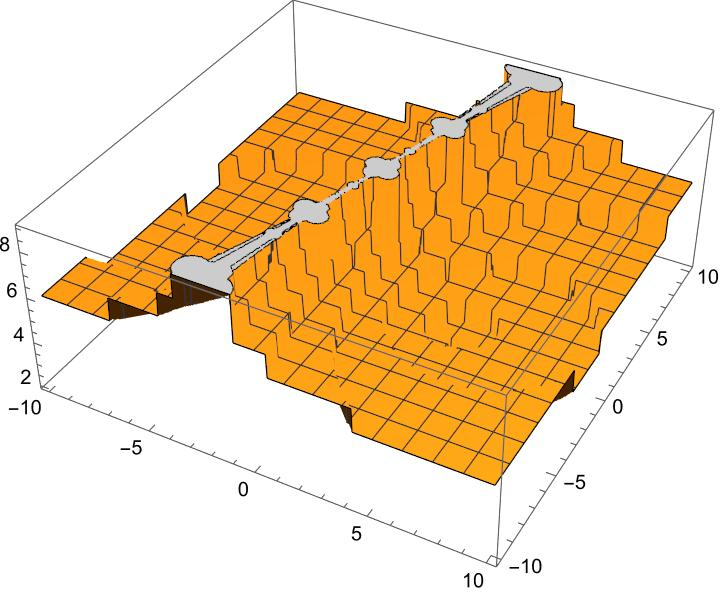
\includegraphics[width=\textwidth]{3D4}
			\caption{Область сходимости метода Ньютона "3D" (аналитическая производная)}
		\end{subfigure}
	\end{figure}

	\begin{figure}[H]
	\centering
	\begin{subfigure}{0.45\textwidth}
		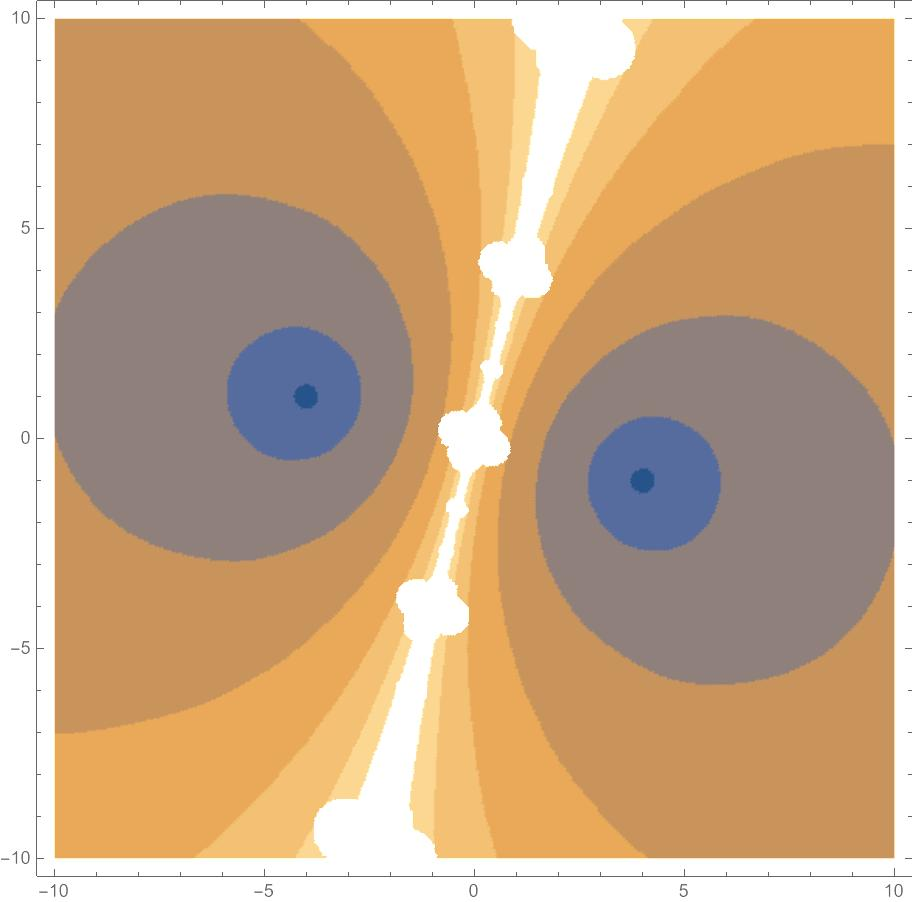
\includegraphics[width=\textwidth]{2D4ch}
		\caption{Область сходимости метода Ньютона "2D" (аналитическая производная)}
	\end{subfigure}
	\hfill
	\begin{subfigure}{0.45\textwidth}
		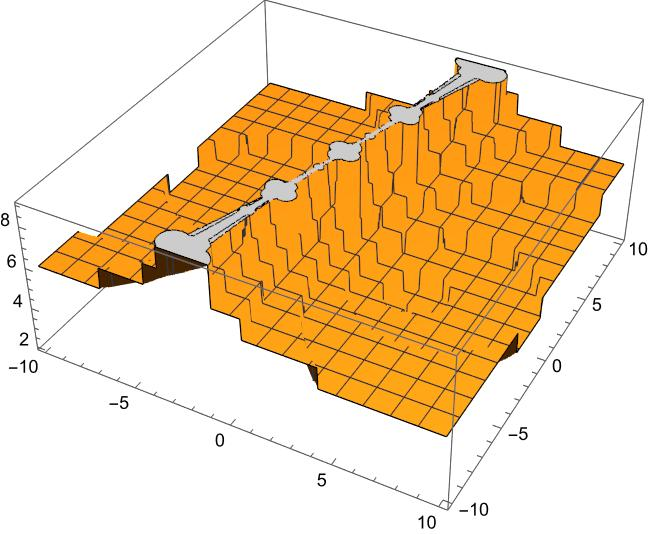
\includegraphics[width=\textwidth]{3D4ch}
		\caption{Область сходимости метода Ньютона "3D" (аналитическая производная)}
	\end{subfigure}
\end{figure}
	
	\newpage
	
	Тест 5
	\[
		\begin{cases}
		x_1^2+x_2^2+x_1+x_2-8=0\\
		x_1^2+x_2^2+x_1x_2-7=0
		\end{cases}
	\]


\begin{figure}[H]
	\centering
	\begin{subfigure}{0.45\textwidth}
		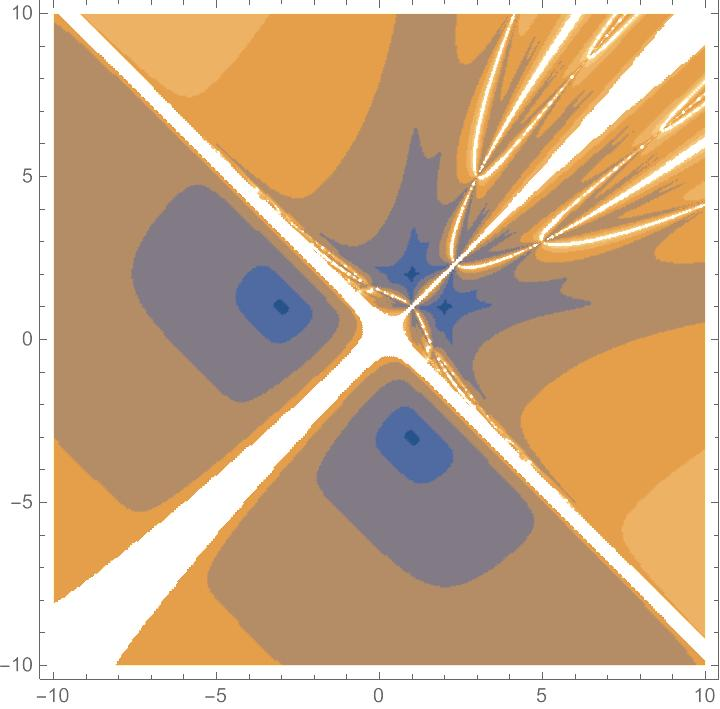
\includegraphics[width=\textwidth]{2D5}
		\caption{Область сходимости метода Ньютона "2D" (аналитическая производная)}
	\end{subfigure}
	\hfill
	\begin{subfigure}{0.45\textwidth}
		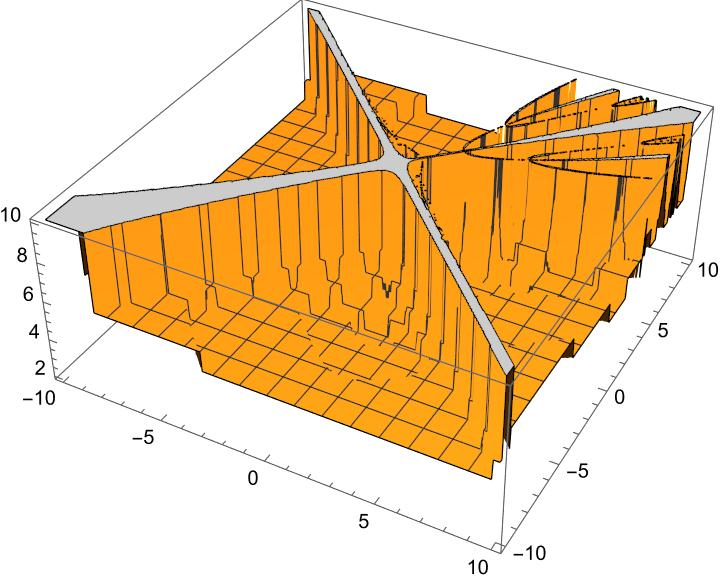
\includegraphics[width=\textwidth]{3D5}
		\caption{Область сходимости метода Ньютона "3D" (аналитическая производная)}
	\end{subfigure}
\end{figure}

\begin{figure}[H]
	\centering
	\begin{subfigure}{0.45\textwidth}
		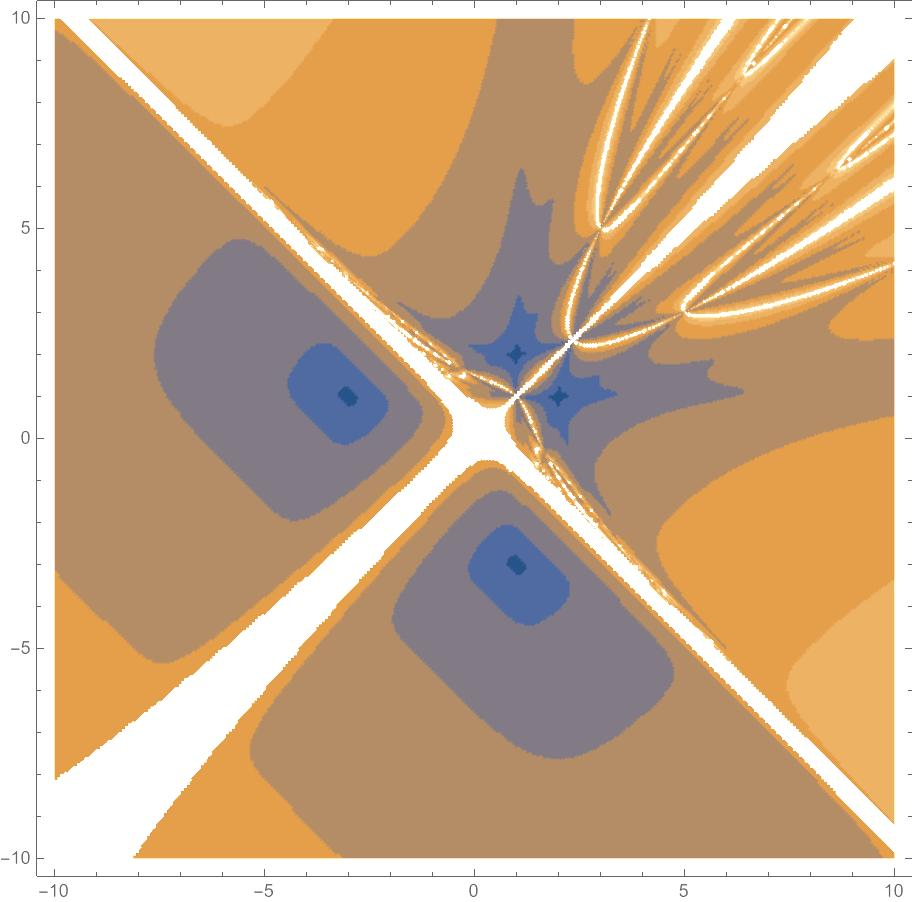
\includegraphics[width=\textwidth]{2D5ch}
		\caption{Область сходимости метода Ньютона "2D" (численная производная)}
	\end{subfigure}
	\hfill
	\begin{subfigure}{0.45\textwidth}
		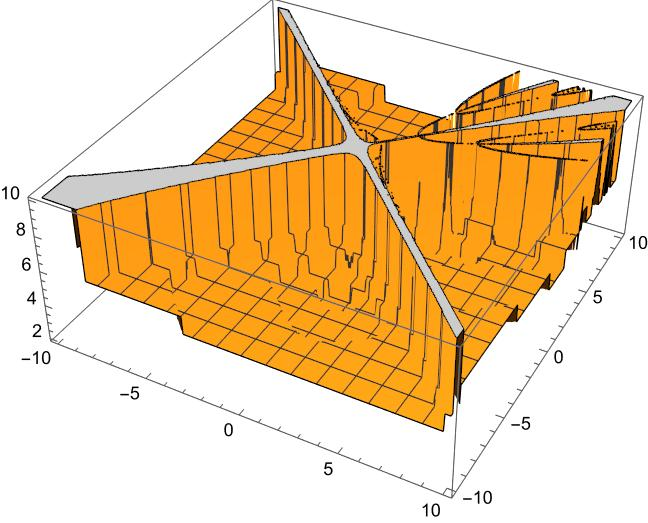
\includegraphics[width=\textwidth]{3D5ch}
		\caption{Область сходимости метода Ньютона "3D" (численная производная)}
	\end{subfigure}
\end{figure}
	
	
	\newpage
	\begin{thebibliography}{1}
		\bibitem{galanin} \textit{Галанин М.П., Савенков Е.Б.} Методы численного анализа математических\\ моделей. М.: Изд-во МГТУ им. Н.Э. Баумана,	2010. 592 с.
		
		
	\end{thebibliography}
	
	
\end{document}
